\subsection{The portfolio}

Table~\ref{tab:studies} lists the \StudiesTotal{} studies in the order their plans were committed. They span
\StudyDomains{} of the \LeadDomains{} fields in the lead database. \StudiesReported{} have reports and 2 are still
running.

The first report appeared on \CalendarFirstReport{}. The other \ReportsAfterFirst{} followed within
\CalendarBulkDays{} days, ending on \CalendarLastReport{}; several studies ran in parallel.

Of the \VerdictsDecided{} decided verdicts, \VerdictSupported{} support the preregistered hypothesis and
\VerdictRefuted{} refute it. \VerdictUnsupported{} are \emph{Unsupported}: the evidence goes against the hypothesis
without meeting the refutation rule. The remaining \VerdictInconclusive{} are \emph{Inconclusive}. One more study, a prospective test, is \emph{Pending} until its outcome data exist in 2027.

\begin{table}[t]
\centering\footnotesize
\caption{The \StudiesTotal{} studies, in order of plan commit. ``Plan first'': git shows the plan committed before
any outcome file. $^\dagger$The plan was committed together with pre-outcome material only (Section~\ref{sec:prereg}).
``Blinding'': how outcomes were kept from the agent before the analysis was fixed (Section~\ref{sec:inventory}).
``Power'': whether the plan stated a power analysis or minimum detectable effect.}
\label{tab:studies}
\begin{tabularx}{\textwidth}{@{}rl X l l l l@{}}
\toprule
\# & Field & Question & Verdict & Plan first & Blinding & Power \\
\midrule
1 & Astronomy & Is the GWTC-4 mass-ratio--spin anticorrelation real? & Inconclusive & \textbf{no} & -- & -- \\
2 & Bioinformatics & Do ClinGen variant-predictor thresholds still hold? & Refuted & yes & -- & -- \\
3 & Climate & Are heat records broken by growing margins? & Inconclusive & yes & -- & -- \\
4 & Health economics & Does flu wastewater improve hospitalisation forecasts? & Unsupported & same commit$^\dagger$ & -- & -- \\
5 & Metascience & Does citing language predict replication outcomes? & Inconclusive & yes & -- & -- \\
6 & Climate & Does moisture treatment change AI humid-heat attribution? & Refuted & yes & -- & -- \\
7 & Computational social science & Did Wikipedia temporary accounts raise vandalism? & Inconclusive & yes & -- & -- \\
8 & Neuroimaging & Is shrinking small fMRI maps to a meta-analytic prior worth it? & Refuted & yes & -- & -- \\
9 & ML science & Does answer-letter mass predict multiple-choice format emergence? & Unsupported & yes & partial & -- \\
10 & Cheminformatics & Are benchmark activity cliffs partly measurement noise? & Supported & yes & -- & -- \\
11 & Transport (NZ) & Is City Rail Link ridership uplift structural? & Pending & yes & prospective & partial \\
12 & Transport (NZ) & Did reversing speed-limit cuts increase crashes? & Inconclusive & same commit$^\dagger$ & sealed & yes \\
13 & Public health (NZ) & Is COVID-19 under-ascertainment greater in deprived towns? & Inconclusive & same commit$^\dagger$ & -- & -- \\
14 & Urban environment (NZ) & Did Auckland's 2016 upzoning cost tree canopy? & Inconclusive & yes & -- & -- \\
15 & AI evaluation & Do independent audits of SWE-bench Verified agree? & Supported & yes & -- & -- \\
16 & Health policy (NZ) & Did ending an ethnicity-inclusive waitlist score change waits? & Inconclusive & yes & partial & -- \\
17 & Seismology & Do neural point processes beat ETAS only via incompleteness? & Supported & yes & -- & -- \\
18 & Quantum simulation & Can one GPU recover 98-qubit peaked-circuit answers? & \emph{in progress} & yes & sealed & -- \\
19 & Formal mathematics & Do self-play provers drift toward vacuous conjectures? & \emph{in progress} & yes & -- & -- \\
\bottomrule
\end{tabularx}

\end{table}

\subsection{Was the plan committed before the outcomes?}
\label{sec:prereg}

Git history shows the plan committed strictly before any results file or report in \PreregPassStrict{} of
\StudiesTotal{} studies. The median gap was \PreregMedianHours{} hours. In the other \PreregSameCommit{}, the plan and
some results files arrived in the same commit, so we inspected those files.
\begin{itemize}
\item \textbf{Three contained only pre-outcome material:}
  \begin{itemize}
  \item pre-period tables and the minimum detectable effect, plus the hash of the sealed post-period file
  (speed limits);
  \item a catchment list (wastewater);
  \item a data-coverage table (FluSight).
  \end{itemize}
\item \textbf{The fourth was the lab's first study (GWTC-4).} Its plan entered git in the same commit as ``full-run
results''. The plan text says it was drafted three weeks earlier, but the public record cannot confirm that. Its
report nevertheless described the study as preregistered. We have added a correction to that report.
\end{itemize}
Counting pre-outcome material as compliant, \PreregPassClassified{} of \StudiesTotal{} plans demonstrably came first.
No plan was edited after its first commit.

\subsection{Which safeguards did the plans actually use?}
\label{sec:inventory}

The safeguards were applied unevenly.

\paragraph{Applied consistently.}
\begin{itemize}
\item Every plan stated a decision rule and was followed by independent review.
\item \InvDisclosure{} plans disclosed what had already been seen (1 partially).
\item \InvDataOpen{} used only data open without registration.
\end{itemize}

\paragraph{Applied unevenly.}
\begin{itemize}
\item \InvValidation{} plans required methods to be validated before the primary analysis, \InvValidationPartial{}
partially, and 2 not at all.
\item Of the 8 plans with several primary tests, \InvMultiplicityYes{} addressed multiplicity.
\end{itemize}

\paragraph{Rarely applied.}
\begin{itemize}
\item \textbf{Power.} Only one plan stated a power analysis or minimum detectable effect before results, and one more did so partially.
\item \textbf{Keeping outcomes away from the agent.} This was done in \InvBlindStrong{} studies: sealed post-period
data with a recorded hash (speed limits), sealed hardware answer strings (quantum), and outcome data that did not yet
exist (City Rail Link). \InvBlindPartial{} more did so in part. In the remaining \InvBlindNone{}, the outcome data
were public and the agent could in principle have analysed them before writing the plan. The plan's disclosure is the
only safeguard there.
\end{itemize}
Only one \emph{decided} study (speed limits) had its outcomes sealed.

\subsection{Deviations}

The two coders identified \DevCodedA{} and \DevCodedB{} deviation entries, differing only in whether one review
paragraph in GWTC-4 counts as a separate entry.
Agreement was:
\begin{itemize}
\item category: $\kappa=\KappaCategory{}$ (\AgreeCategory{} raw agreement);
\item trigger: $\kappa=\KappaTrigger{}$;
\item timing: $\kappa=\KappaTiming{}$;
\item verdict relevance: $\kappa=\KappaVerdictRelevance{}$.
\end{itemize}

\DevDisagreeEntries{} entries had at least one disagreement. We settled these with three fixed rules: category
follows the cause; verdict relevance takes the cautious side; timing is ``unclear'' if either coder said so. Each
decision is logged with its reason. After adjudication there are \DevTotal{} entries across \DevStudies{} studies
(Figure~\ref{fig:dev}).

\paragraph{Categories.} The largest categories were added secondary analyses (\DevCFive{}), clarifications
(\DevCSeven{}), bug or numerical fixes (\DevCOne{}), environment and logistics (\DevCSix{}), changes to the primary
analysis specification (\DevCThree{}) and data problems (\DevCTwo{}). \DevCEight{} entries withdrew or corrected a
claim, and \DevCFour{} changed a decision rule or its thresholds.

\paragraph{Triggers and timing.} The executing agent triggered \DevTOne{} entries, validation checks \DevTTwo{}, the
independent reviewer \DevTThree{}, and external events \DevTFour{}. \DevAfter{} entries were made after the primary
outcome had been seen, \DevBefore{} before, and \DevUnclearTiming{} could not be dated.

\paragraph{Verdict relevance.} \DevVerdictRelevant{} entries (\DevVerdictRelevantPct{}) were judged capable of
changing the verdict, and \DevRelevantAfter{} of them were made after the outcome was seen. Those are the entries a
reader should scrutinise, and each is in the public log with its reason. Most correct errors found by validation or
review.

\paragraph{Decision-rule changes.} Three entries changed a decision rule:
\begin{itemize}
\item one in GWTC-4, later judged post hoc by the study's own final audit;
\item one in the City Rail Link study, rewritten after review but before any outcome data existed;
\item a tie-breaking rule in the quantum study, fixed before any candidate answer was scored.
\end{itemize}

\begin{figure}[t]
\centering
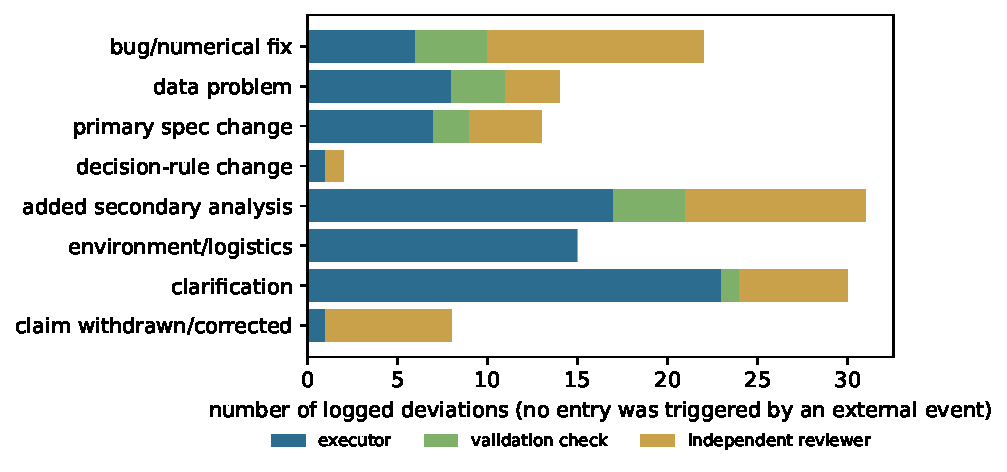
\includegraphics[width=0.85\textwidth]{figures/deviations.pdf}
\caption{Logged deviations by category and trigger (adjudicated codes).}
\label{fig:dev}
\end{figure}

\subsection{What independent review changed}

Every review asked for changes before publication. \ReviewFixFirst{} of \ReviewStudies{} said ``fix first'' and the
rest ``publish with edits''. \ReviewConfirmation{} studies had a confirmation pass.

The coders agreed closely on outcomes but not on how many issues each review raised:
\begin{itemize}
\item agreement on whether the headline changed was \AgreeHeadlineChanged{}, and on whether the verdict changed
\AgreeVerdictChanged{};
\item agreement on the exact number of issues was only \ReviewIssuesExactAgree{}, so we report both coders' totals.
\end{itemize}
They counted \ReviewIssuesTotal{} and \ReviewIssuesTotalB{} substantive issues (medians \ReviewIssuesMedian{} and
\ReviewIssuesMedianB{} per study), which break down as follows:
\begin{itemize}
\item analysis or model errors: \ReviewRTwo{} and \ReviewRTwoB{};
\item computational or numerical errors: \ReviewROne{} and \ReviewROneB{};
\item overclaiming: \ReviewRFour{} and \ReviewRFourB{};
\item missing analyses: \ReviewRFive{} and \ReviewRFiveB{};
\item documentation: \ReviewRSix{} and \ReviewRSixB{};
\item leakage or blinding: \ReviewRThree{} each.
\end{itemize}

After adjudication, review changed the headline estimate in \ReviewHeadlineChanged{} studies:
\begin{itemize}
\item a false-positive rate in GWTC-4 moved from 0.24 to 0.010;
\item the seismology recovery fraction at Norcia moved from 0.51 to 0.88, after the reviewer found a local optimum;
\item in the cheminformatics study, the headline share of the activity-cliff gap reproduced by noise alone moved from 171\% (from an over-dispersed noise model) to ``about 100--115\%''.
\item the upzoning estimate shifted.
\end{itemize}
It changed the verdict in \ReviewVerdictChanged{} studies:
\begin{itemize}
\item GWTC-4, from a confirmation to ``indeterminate'';
\item the citation-context study, from a refutation to ``uninformative'', after its positive control failed.
\end{itemize}
In one further study the pre-review draft was never committed, so whether its verdict changed cannot be determined.

\subsection{Do the numbers in reports trace to results?}

The reports contain \NumAll{} numbers, of which \NumSubstantive{} are substantive (decimals, percentages or integers
of at least 100). Of these, \NumTracedSubst{} match a value in the study's own results, plan or deviation log
(Figure~\ref{fig:numbers}). That figure is misleading. Matched against \emph{other} studies' results, a report's
numbers still ``trace'' \NumChanceAll{} of the time on average, because results files hold thousands of values.

Tracing becomes informative only with more significant figures:
\begin{itemize}
\item at three significant figures (\NumNThree{} numbers), \NumOwnThree{} trace against a chance rate of
\NumChanceThree{}, which corrects to about \NumCorrectedThree{};
\item at four, \NumOwnFour{} trace against \NumChanceFour{};
\item at five or more (\NumNFive{} numbers, mostly large counts), only \NumOwnFive{} trace.
\end{itemize}
\paragraph{Untraced numbers.} Both coders classified a seeded sample of \UntracedN{} untraced substantive numbers
(up to 10 per report; drawn before the matcher fix in \texttt{audit/deviations.md}~A8).
\begin{itemize}
\item \textbf{Inconsistent with the results:} \UntracedUFiveAny{}. Neither coder found any.
\item \textbf{Untraceable:} \UntracedUFourBoth{}, the same three for both coders. All three are numbers the
independent reviewer computed in its own scratch code and that were never saved: two canopy percentages from a
point-density thinning check, and a likelihood re-integration tolerance.
\item \textbf{From cited literature or data documentation:} \UntracedUTwo{}.
\item \textbf{Legitimately sourced:} the remaining \UntracedOneThree{} were arithmetic on traced numbers, design
parameters or sample counts. The coders differed only on which of these two classes \UntracedOneThreeDisagree{}
belonged to ($\kappa=\UntracedKappa{}$ overall).
\end{itemize}

Outside the sample, coder~A found one real error while recomputing a range. A report printed ``$-1.3$ to $+1.5$''
where the data give $-1.25$ to $+1.449$, so the upper end had been rounded twice. The report has been corrected.


\begin{figure}[t]
\centering
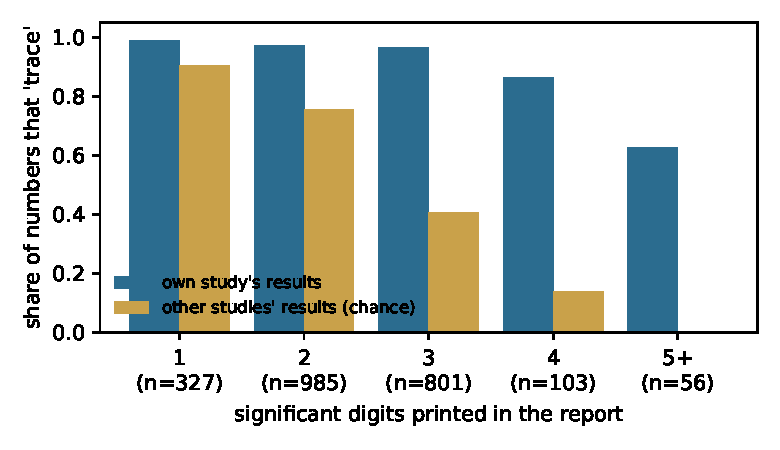
\includegraphics[width=0.62\textwidth]{figures/number_tracing.pdf}
\caption{Share of report numbers that match a value in the study's own results (blue) and, as a chance control, in
other studies' results (gold), by significant figures printed.}
\label{fig:numbers}
\end{figure}

\subsection{References}

All \RefArxiv{} arXiv identifiers cited in leads, plans and reports resolve. \RefDoiOKRaw{} of \RefDoi{} DOIs resolve
automatically; the other two resolve once parsing errors are fixed (a version suffix, and a truncation at a
parenthesis). This checks that the references exist, not that they say what they are cited for.

\subsection{Scout estimates against outcomes}

The scouts estimated a median of \ScoutDaysMedian{} days per study (\ScoutDaysTotal{} days in total for the reported
studies). Neither git history nor the session transcripts give a reliable measure of effort per study:
\begin{itemize}
\item commits were made in bursts;
\item studies ran in parallel;
\item tool calls rarely name the study they belong to.
\end{itemize}
The calendar alone, however, shows effort was overestimated by an order of magnitude or more.

Value and cost scores did not separate verdicts. The mean value score was 6.0--6.7 for every verdict
(\texttt{audit/F\_verdict\_by\_scores.csv}).
